%%%%%%%%%%%%%%%%%
% This is an example CV created using altacv.cls (v1.1, 21 November 2016) written by
% LianTze Lim (liantze@gmail.com), based on the 
% Cv created by BusinessInsider at http://www.businessinsider.my/a-sample-resume-for-marissa-mayer-2016-7/?r=US&IR=T
% 
%% It may be distributed and/or modified under the
%% conditions of the LaTeX Project Public License, either version 1.3
%% of this license or (at your option) any later version.
%% The latest version of this license is in
%%    http://www.latex-project.org/lppl.txt
%% and version 1.3 or later is part of all distributions of LaTeX
%% version 2003/12/01 or later.
%%%%%%%%%%%%%%%%

%% If you want to use \orcid or the
%% academicons icons, add "academicons"
%% to the \documentclass options. 
%% Then compile with XeLaTeX or LuaLaTeX.
% \documentclass[10pt,a4paper,academicons]{altacv}
\documentclass[10pt,a4paper]{altacv}

%% AltaCV uses the fontawesome and academicon fonts
%% and packages. 
%% See texdoc.net/pkg/fontawecome and http://texdoc.net/pkg/academicons for full list of symbols.
%% When using the "academicons" option,
%% Compile with LuaLaTeX for best results. If you
%% want to use XeLaTeX, you may need to install
%% Academicons.ttf in your operating system's font %% folder.


% Change the page layout if you need to
\geometry{left=1cm,right=9cm,marginparwidth=6.8cm,marginparsep=1.2cm,top=1cm,bottom=1cm}

% Change the font if you want to.

% If using pdflatex:
\usepackage[utf8]{inputenc}
\usepackage[T1]{fontenc}
\usepackage[default]{lato}
\usepackage{enumitem} % For customizing lists
\usepackage{pgfplots} % Para gráficos de barras
\pgfplotsset{compat=1.17}
% Colores para el gráfico de barras (paleta azul-verde)
\definecolor{colorB2B}{HTML}{1A5276}
\definecolor{colorProspeccion}{HTML}{1E8C8C}
\definecolor{colorCRM}{HTML}{48B4A0}
\definecolor{colorCierre}{HTML}{6BC9A6}
\definecolor{colorDificultades}{HTML}{8FD9B6}
\definecolor{colorPruebas}{HTML}{B5E7A0}

% If using xelatex or lualatex:
% \setmainfont{Lato}

% Change the colours if you want to
\definecolor{VividPurple}{HTML}{1B4A5C}
\definecolor{SlateGrey}{HTML}{2E2E2E}
\definecolor{LightGrey}{HTML}{666666}
\colorlet{heading}{VividPurple}
\colorlet{accent}{VividPurple}
\colorlet{emphasis}{SlateGrey}
\colorlet{body}{LightGrey}

% Change the bullets for itemize and rating marker
% for \cvskill if you want to
\renewcommand{\itemmarker}{{\small\textbullet}}
\renewcommand{\ratingmarker}{\faCircle}

%% sample.bib contains your publications
% \addbibresource{sample.bib} % Comentado - no se usan publicaciones

\begin{document}
\name{Ana María \newline Albarracín Noreña}
  \tagline{ Ejecutiva Comercial B2B}
% Cropped to square from https://en.wikipedia.org/wiki/Marissa_Mayer#/media/File:Marissa_Mayer_May_2014_(cropped).jpg, CC-BY 2.0
\photo{5.5cm}{me}
% Personal info without bullet points
\personalinfo{%
  \textcolor{accent}{\faEnvelope}\hspace{0.5em}amalbarracin5@gmail.com \\
  \textcolor{accent}{\faPhone}\hspace{0.5em}(+57) 312 825 5775 \\
  \textcolor{accent}{\faLinkedin}\hspace{0.5em}linkedin.com/in/ana-maria-albarracin \\
  \textcolor{accent}{\faMapMarker}\hspace{0.5em}Tarjeta profesional: 26272
}

%% Make the header extend all the way to the right, if you want. Extend the right margin by 8cm (=6.8cm marginparwidth + 1.2cm marginparsep)
\begin{adjustwidth}{}{-7.2 cm}
\makecvheader
\end{adjustwidth}

%% Provide the file name containing the sidebar contents as an optional parameter to \cvsection.
%% You can always just use \marginpar{...} if you do
%% not need to align the top of the contents to any
%% \cvsection title in the "main" bar.
%\cvevent{Consultant Engineer }{Contact and Business IT Ltda}{April 2014 -- March 2014}{Bogota, Colombia}
%Test analyst for banking internet platform.
%\divider



% \divider

% \cvevent{Product Engineer}{Google}{23 June 1999 -- 2001}{Palo Alto, CA}

% \begin{itemize}
% \item Joined the company as employe \#20 and female employee \#1
% \item Developed targeted advertisement in order to use user's search queries and show them related ads
% \end{itemize}
\cvsection[page1sidebar]{Experiencia Laboral}
\cvevent{Ejecutiva Comercial}{Meico Solar}{Mayo 2024--Actualidad}{Bogotá, Colombia}

\begin{itemize}
\item Gestión comercial integral: prospección, identificación de necesidades, cotización, seguimiento estratégico y cierre de ventas con acompañamiento postventa.
\item Realización de visitas de relacionamiento en Bogotá y el Eje Cafetero para fortalecer vínculos con clientes actuales y potenciales.
\item Búsqueda de nuevas oportunidades comerciales basadas en el análisis de datos de grandes clientes del sector, con seguimiento estructurado y propuesta de estrategias de abordaje.
\item Análisis del mercado y mantenimiento del CRM para identificar oportunidades.
\end{itemize}

\cvevent{Asesora Técnica Comercial}{Olaflex SAS}{Julio 2022--Mayo 2024}{Bogotá, Colombia}

\begin{itemize}
\item Gestión de ventas de productos de poliuretano, incluyendo visitas y seguimiento a clientes.
\item Propuesta de desarrollos a medida según el uso final del cliente, incluyendo soporte técnico en planta, pruebas de desempeño y formulación de soluciones personalizadas.
\item Elaboración de planes de marketing y proyección de presupuestos.
\item Coordinación de exportaciones, el manejo de documentación legal y aduanera.
\end{itemize}

\cvevent{Asesora Comercial}{Química MG}{Enero 2022--Julio 2022}{Bogotá, Colombia}

\begin{itemize}
\item Participación en licitaciones y proyectos de ingeniería.
\item Elaboración de propuestas comerciales y seguimiento a clientes.
\end{itemize}

\cvevent{Gestora de Proyectos}{Grupo Coral SAS}{Enero 2020--Agosto 2021}{Bogotá, Colombia}

\begin{itemize}
\item Elaboración de propuestas técnico-comerciales para clientes del sector público y privado.
\item Apoyo en procesos licitatorios y desarrollo de nuevos negocios.
\end{itemize}

% Se dejo un espacio de un centimetro, no olvidar ----------------------------------------------------------------------------------------------------------------------------------------------
\newpage
\cvsection[page2sidebar]{Un día en mi vida}
\begin{adjustwidth}{}{-7.2cm}
\begin{center}
\hspace{-7cm}\wheelchart{2cm}{0.4cm}{%
35/12em/accent/Trabajar,
20/10em/accent!60/Ocio,
15/8em/accent!30/Descansar,
10/14em/accent!10/Compartir con mi gato,
10/9em/accent!40/Ejercicio,
10/13em/accent!50/Familia y amigos}
\end{center}
\end{adjustwidth}

\cvsection{Competencias por Empresa}
\begin{adjustwidth}{}{-7.2cm}
\begin{center}
\hspace{-7.5cm}
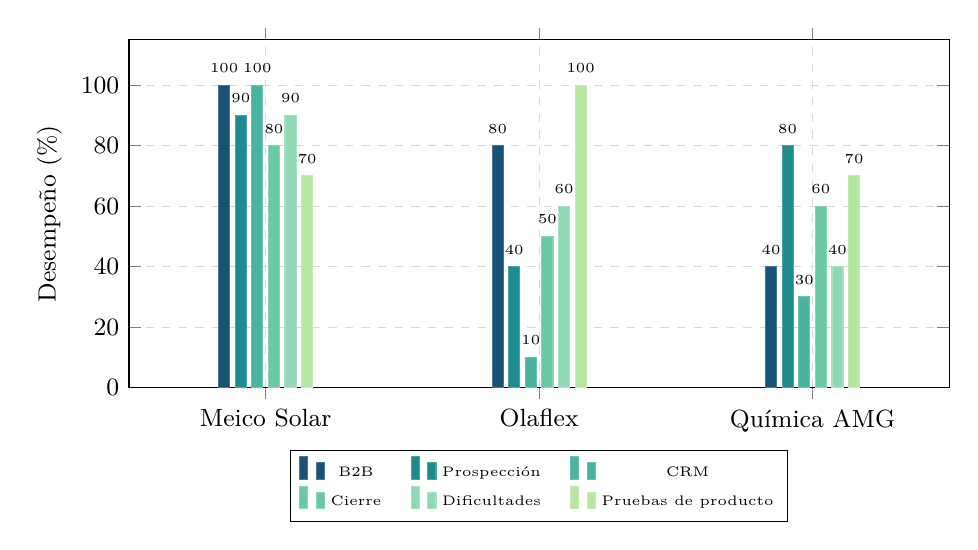
\begin{tikzpicture}
\begin{axis}[
    ybar,
    width=12cm,
    height=6cm,
    bar width=4pt,
    ylabel={Desempeño (\%)},
    ymin=0,
    ymax=115,
    ytick={0,20,40,60,80,100},
    symbolic x coords={Meico Solar, Olaflex, Química AMG},
    xtick=data,
    x tick label style={font=\small},
    y tick label style={font=\small},
    ylabel style={font=\small},
    legend style={
        at={(0.5,-0.18)},
        anchor=north,
        legend columns=3,
        font=\tiny,
        /tikz/every even column/.append style={column sep=0.3cm}
    },
    nodes near coords,
    nodes near coords style={font=\tiny, above},
    every node near coord/.append style={yshift=1pt},
    enlarge x limits=0.25,
    grid=major,
    grid style={dashed, gray!30},
]
% B2B - Azul oscuro
\addplot[fill=colorB2B, draw=colorB2B!80] coordinates {
    (Meico Solar,100) (Olaflex,80) (Química AMG,40)
};
% Prospección - Naranja
\addplot[fill=colorProspeccion, draw=colorProspeccion!80] coordinates {
    (Meico Solar,90) (Olaflex,40) (Química AMG,80)
};
% CRM - Verde
\addplot[fill=colorCRM, draw=colorCRM!80] coordinates {
    (Meico Solar,100) (Olaflex,10) (Química AMG,30)
};
% Cierre - Morado
\addplot[fill=colorCierre, draw=colorCierre!80] coordinates {
    (Meico Solar,80) (Olaflex,50) (Química AMG,60)
};
% Dificultades - Rojo
\addplot[fill=colorDificultades, draw=colorDificultades!80] coordinates {
    (Meico Solar,90) (Olaflex,60) (Química AMG,40)
};
% Pruebas de producto
\addplot[fill=colorPruebas, draw=colorPruebas!80] coordinates {
    (Meico Solar,70) (Olaflex,100) (Química AMG,70)
};
\legend{B2B, Prospección, CRM, Cierre, Dificultades, Pruebas de producto}
\end{axis}
\end{tikzpicture}
\end{center}
\end{adjustwidth}

\cvsection{Referencias}
\cvref{Daniela Perdomo Morales, Ejecutiva comercial, Biopolar}{+57 313 8653659}{}
\divider

\cvref{Juan David Tuta Botero, Director de ingeniería, Abatech}{+57 3016395759}{}

\vspace{1cm}

\end{document}
